\section{Versuchsaufbau}
\label{sec:Versuchaufbau}

Mit dem in Abbildung \ref{fig:aufbau_1} dargestellten Versuch wird der normale und der anomale Zeeman-Effekt nachgewiesen.

\begin{figure}[H]
  \centering
  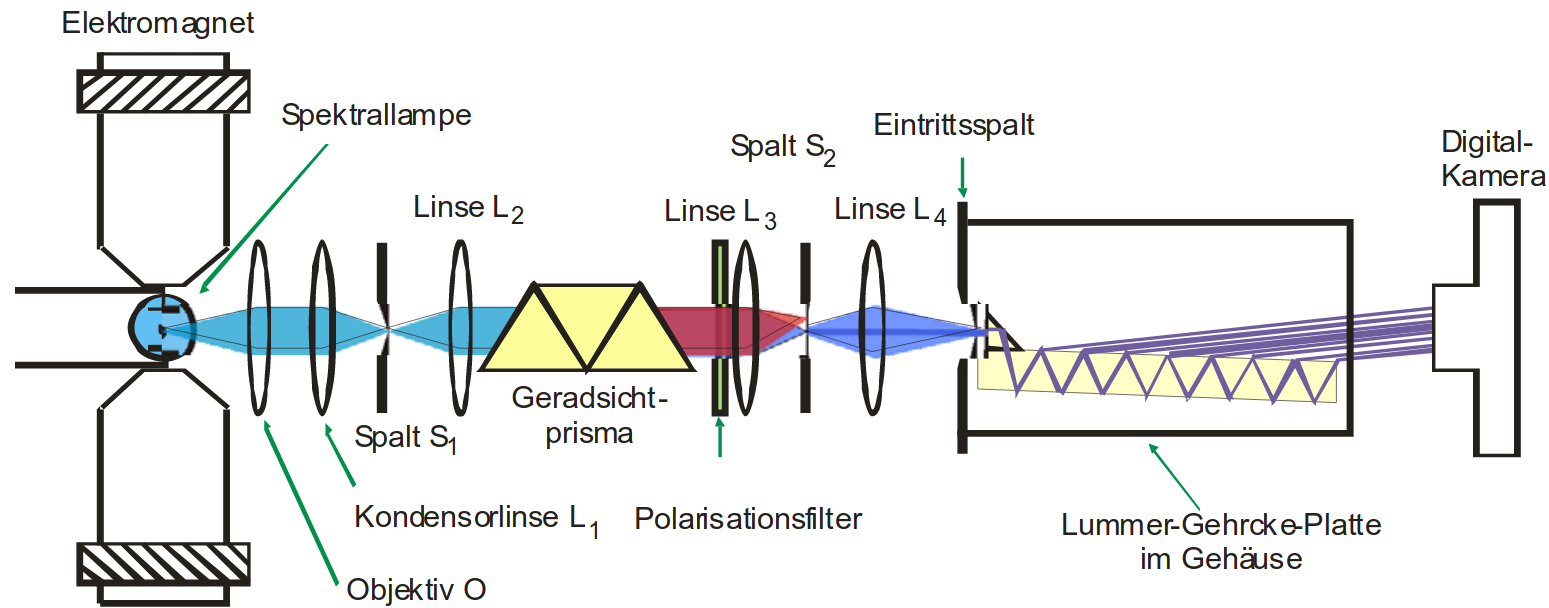
\includegraphics[width=.75\textwidth]{ressources/Aufbau.png}
  \caption{Aufbau des durchgeführten Versuchs\cite{skript}.}
  \label{fig:aufbau_1}
\end{figure}

Für den Versuch wird eine Cd-Lampe verwendet. Anhand der blauen Spektrallinien kann der anomale und anhand der roten Spektrallinien der normale Zeeman-Effekt beobachtet werden. Ursache für die Aufspaltung der Niveaus ist ein Elektromagnet. Die abgestrahlten Spektrallinien werden fokussiert und parallelisiert. Mit einem Geradsichtprisma erfolgt eine Aufspaltung parallel zur optischen Achse in Abhängigkeit der Wellenlänge $\lambda$. Um zwischen den $\pi$- und $\sigma_\pm$-Komponenten zu unterscheiden, wird ein Polarisationsfilter verwendet. Schlussendlich wird die Spektrallinie auf eine Lummer-Gehrcke-Platte gelegt und das Interferenzmuster mit einer Digitalkamera aufgezeichnet.

\subsection{Lummer-Gehrcke-Platte}

Bei Lummer-Gehrcke-Platte werden planparallel Platten für ein maximales Auflösungsvermögen verwendet. Über ein Prisma wird der Lichtstrahl in die planparallelen Platten gelenkt. Innerhalb dieser, wird der Strahl mehrfach reflektiert. Jedoch tritt bei jeder Reflexion ein kleiner Teil des Lichts aus den Platten aus. Dadurch entstehen mehrere Strahlenbündel die untereinander interferieren. In Abbildung \ref{fig:aufbau_2} ist die Zeichnung eine Lummer-Gehrcke-Platte dargestellt. 

\begin{figure}[H]
  \centering
  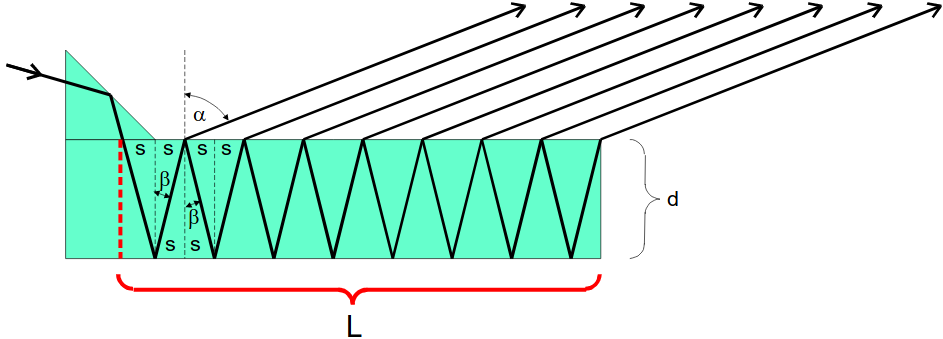
\includegraphics[width=.75\textwidth]{ressources/Platte.png}
  \caption{Aufbaus einer Lummer-Gehrcke-Platte\cite{skript}.}
  \label{fig:aufbau_2}
\end{figure}

Für konstruktive Interferenz muss die Bedingung
\begin{align}
	2d\cos{\theta}=n\lambda
\end{align}
erfüllt sein. Dabei bezeichnet $d$ die Dicke die Lummer-Gehrcke-Platte, $n$ die Interferenzordnung, $\theta$ des Einfallswinkel des Lichts und $\lambda$ die Wellenlänge.
Unter Verwendung von monochromatischem Licht erzeugt die Lummer-Gehrcke-Platte einen Interferenzstreifen mit dem Gangunterschied $\lambda$. Das eingeschaltete Magnetfeld verursacht jedoch eine Verschiebung der Wellenlänge $\delta \lambda$ und dadurch eine Verschiebung des Interferenzstreifens $\delta s$
Damit es zur keiner Überlagerung kommt, darf eine maximale Wellenlängendifferenz von
\begin{align}
	\Delta \lambda_D=\frac{\lambda^2}{2d}\sqrt{\frac{1}{n^2-1}}\;.
\end{align}

Das Auflösungsvermögen kann wie folgt bestimmt werden
\begin{align}
	A=\frac{\lambda}{\Delta\lambda}=\frac{L}{\Delta \lambda}(n^2-1)\;.
\end{align}
Dabei beschreibt $L$ die Länge der Lummer-Gehrcke-Platte und $n$ des Brechungsindex.